
\title{Lab 5 - SDP}
\author{Jacopo Nasi\\
        Stud. ID: 255320\\
        Politecnico di Torino}
\date{\bigskip\bigskip\today}

\documentclass[12pt]{article}
\usepackage[utf8]{inputenc}
\usepackage[italian]{babel}
\usepackage{geometry}
\usepackage{indentfirst} % First line indent
\usepackage{mathtools}
\usepackage{wrapfig}
\usepackage[usenames, dvipsnames]{color}
\usepackage{float}
\usepackage{amssymb}
\usepackage{ifsym}
\usepackage{multicol}
% Misure Documento
\geometry{ a4paper, total={170mm,257mm},left=35mm, right=35mm, top=32mm, bottom=32mm }

\usepackage{xcolor}
\usepackage{listings}

\definecolor{mGreen}{rgb}{0,0.6,0}
\definecolor{mGray}{rgb}{0.5,0.5,0.5}
\definecolor{mPurple}{rgb}{0.58,0,0.82}
\definecolor{backgroundColour}{rgb}{0.95,0.95,0.92}

\lstdefinestyle{CStyle}{
    backgroundcolor=\color{backgroundColour},
    commentstyle=\color{mGreen},
    keywordstyle=\color{magenta},
    numberstyle=\tiny\color{mGray},
    stringstyle=\color{mPurple},
    basicstyle=\footnotesize,
    breakatwhitespace=false,
    breaklines=true,
    captionpos=b,
    keepspaces=true,
    numbers=left,
    numbersep=5pt,
    showspaces=false,
    showstringspaces=false,
    showtabs=false,
    tabsize=2,
    language=C
}

\begin{document}

\begin{figure}
  \centering
  
\includegraphics[width=10cm]{images/polito.pdf}
\end{figure}

\maketitle
\newpage

\section{Genesis}
The following text is based on *nix environment. This report is written based on laboratory experience and the \textit{http://www.jamesmolloy.co.uk} tutorial.

\subsection{Boot Code}
The main part of the boot code is written in C, the assembly part are in the INTEL form. The \textit{boot.s} file is used to call the main of the C program, the other part are used for the multiboot header.\\
Multiboot is a standard to which GRUB expects a kernel to comply. This multiboot allows to inform the system which kernel must load at the system boot.\\
The first important command are:
\begin{lstlisting}[style=CStyle]
  push EBX
  cli
  call main
  jump $
\end{lstlisting}
The first line push the content of EBX, the pointer to the multiboot part, to the stack, disable interrupts (CLI), call a 'main' C function, then enter an infinite loop. Since the interface between a C function and the assembly is made by pushing the parameters in the stack, the line 1 is used to passing a paramter to the function main(). The result of the function instead will be stored in the EAX register.\\
The main code is really simple:
\begin{lstlisting}[style=CStyle]
  /* main.c -- Defines the C-code kernel entry point,
  calls initialisation routines.
  Made for JamesM's tutorials */

  int main(struct multiboot *mboot_ptr)
  {
    // All our initialisation calls will go in here.
    return 0xDEADBABA;
  }
\end{lstlisting}

\section{GDT and IDT}
The GDT and the IDT are descriptor tables. They are arrays of flags and bit values describing the operation of either the segmentation system (in the case of the GDT), or the interrupt vector table (IDT).
\subsection{The GDT}
The x86 architecture has two methods of memory protection and of providing virtual memory - segmentation and paging.\\
With segmentation, every memory access is evaluated with respect to a segment. That is, the memory address is added to the segment's base address, and checked against the segment's length. You can think of a segment as a window into the address space - The process does not know it's a window, all it sees is a linear address space starting at zero and going up to the segment length.\\
With paging, the address space is split into (usually 4KB, but this can change) blocks, called pages. Each page can be mapped into physical memory - mapped onto what is called a 'frame'. Or, it can be unmapped. Like this you can create virtual memory spaces.\\
Both of these methods have their advantages, but paging is much better. Segmentation is, although still usable, fast becoming obsolete as a method of memory protection and virtual memory. In fact, the x86-64 architecture requires a flat memory model (one segment with a base of 0 and a limit of 0xFFFFFFFF) for some of it's instructions to operate properly.\\

The structure of the GDT is the following:
\begin{lstlisting}[style=CStyle]
  // This structure contains the value of one GDT entry.
  // We use the attribute 'packed' to tell GCC not to change
  // any of the alignment in the structure.
  struct gdt_entry_struct
  {
     u16int limit_low;           // The lower 16 bits of the limit.
     u16int base_low;            // The lower 16 bits of the base.
     u8int  base_middle;         // The next 8 bits of the base.
     u8int  access;              // Access flags, determine what ring this segment can be used in.
     u8int  granularity;
     u8int  base_high;           // The last 8 bits of the base.
  } __attribute__((packed));
  typedef struct gdt_entry_struct gdt_entry_t;
\end{lstlisting}
\begin{figure}[H]
  \centering
  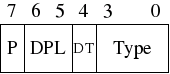
\includegraphics[width=5cm]{images/gdt.png}
  \caption{Access byte format GDT}
\end{figure}
\begin{figure}[H]
  \centering
  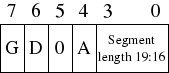
\includegraphics[width=5cm]{images/gdt2.png}
  \caption{Granularity byte format GDT}
\end{figure}
The byte are:
\begin{itemize}
  \item \textbf{P}: Is segment present? (1 = Yes)
  \item \textbf{DPL}:Descriptor privilege level - Ring 0 - 3.
  \item \textbf{DT}:Descriptor type
  \item \textbf{Type}:Segment type - code segment / data segment.
  \item \textbf{G}:Granularity (0 = 1 byte, 1 = 1kbyte)
  \item \textbf{D}:Operand size (0 = 16bit, 1 = 32bit)
  \item \textbf{0}:Should always be zero.
  \item \textbf{A}:Available for system use (always zero).
\end{itemize}

\subsection{Utilization}
The following line report some of the function used over the defined structure:
\begin{lstlisting}[style=CStyle]
  // Initialisation routine - zeroes all the interrupt service routines,
  // initialises the GDT and IDT.
  void init_descriptor_tables()
  {
   // Initialise the global descriptor table.
   init_gdt();
  }

  static void init_gdt()
  {
   gdt_ptr.limit = (sizeof(gdt_entry_t) * 5) - 1;
   gdt_ptr.base  = (u32int)&gdt_entries;

   gdt_set_gate(0, 0, 0, 0, 0);                // Null segment
   gdt_set_gate(1, 0, 0xFFFFFFFF, 0x9A, 0xCF); // Code segment
   gdt_set_gate(2, 0, 0xFFFFFFFF, 0x92, 0xCF); // Data segment
   gdt_set_gate(3, 0, 0xFFFFFFFF, 0xFA, 0xCF); // User mode code segment
   gdt_set_gate(4, 0, 0xFFFFFFFF, 0xF2, 0xCF); // User mode data segment

   gdt_flush((u32int)&gdt_ptr);
  }

  // Set the value of one GDT entry.
  static void gdt_set_gate(s32int num, u32int base, u32int limit, u8int access, u8int gran)
  {
   gdt_entries[num].base_low    = (base & 0xFFFF);
   gdt_entries[num].base_middle = (base >> 16) & 0xFF;
   gdt_entries[num].base_high   = (base >> 24) & 0xFF;

   gdt_entries[num].limit_low   = (limit & 0xFFFF);
   gdt_entries[num].granularity = (limit >> 16) & 0x0F;

   gdt_entries[num].granularity |= gran & 0xF0;
   gdt_entries[num].access      = access;
  }
\end{lstlisting}

\subsection{The IDT}
There are times when you want to interrupt the processor. You want to stop it doing what it is doing, and force it to do something different. An example of this is when an timer or keyboard interrupt request (IRQ) fires. An interrupt is like a POSIX signal - it tells you that something of interest has happened. The processor can register 'signal handlers' (interrupt handlers) that deal with the interrupt, then return to the code that was running before it fired. Interrupts can be fired externally, via IRQs, or internally, via the 'int n' instruction. There are very useful reasons for wanting to do fire interrupts from software, but that's for another chapter!\\

The Interrupt Descriptor Table tells the processor where to find handlers for each interrupt. It is very similar to the GDT. It is just an array of entries, each one corresponding to an interrupt number. There are 256 possible interrupt numbers, so 256 must be defined. If an interrupt occurs and there is no entry for it (even a NULL entry is fine), the processor will panic and reset.

\subsection{Faults, traps and exceptions}
The processor will sometimes need to signal your kernel. Something major may have happened, such as a divide-by-zero, or a page fault. To do this, it uses the first 32 interrupts. It is therefore doubly important that all of these are mapped and non-NULL - else the CPU will triple-fault and reset (bochs will panic with an 'unhandled exception' error).

The special, CPU-dedicated interrupts are shown below.
\begin{multicols}{2}
  \begin{itemize}
    \item 0 - Division by zero exception
    \item 1 - Debug exception
    \item 2 - Non maskable interrupt
    \item 3 - Breakpoint exception
    \item 4 - 'Into detected overflow'
    \item 5 - Out of bounds exception
    \item 6 - Invalid opcode exception
    \item 7 - No coprocessor exception
    \item 8 - Double fault (pushes an error code)
    \item 9 - Coprocessor segment overrun
    \item 10 - Bad TSS (pushes an error code)
    \item 11 - Segment not present (pushes an error code)
    \item 12 - Stack fault (pushes an error code)
    \item 13 - General protection fault (pushes an error code)
    \item 14 - Page fault (pushes an error code)
    \item 15 - Unknown interrupt exception
    \item 16 - Coprocessor fault
    \item 17 - Alignment check exception
    \item 18 - Machine check exception
    \item 19-31 - Reserved
  \end{itemize}
\end{multicols}

\section{IRQs and the PIT}
\subsection{Interrupt requests}
There are several methods for communicating with external devices. Two of the most useful and popular are polling and interrupting.
\begin{itemize}
  \item Polling: Spin in a loop, occasionally checking if the device is ready.
  \item Interrupts: Do lots of useful stuff. When the device is ready it will cause a CPU interrupt, causing your handler to be run.
\end{itemize}
As can probably be gleaned from my biased descriptions, interrupting is considered better for many situations. Polling has lots of uses - some CPUs may not have an interrupt mechanism, or you may have many devices, or maybe you just need to check so infrequently that it's not worth the hassle of interrupts. Any rate, interrupts are a very useful method of hardware communication. They are used by the keyboard when keys are pressed, and also by the programmable interval timer (PIT).\\
The low-level concepts behind external interrupts are not very complex. All devices that are interrupt-capable have a line connecting them to the PIC (programmable interrupt controller). The PIC is the only device that is directly connected to the CPU's interrupt pin. It is used as a multiplexer, and has the ability to prioritise between interrupting devices. It is, essentially, a glorified 8-1 multiplexer. At some point, someone somewhere realised that 8 IRQ lines just wasn't enough, and they daisy-chained another 8-1 PIC beside the original. So in all modern PCs, you have 2 PICs, the master and the slave, serving a total of 15 interruptable devices (one line is used to signal the slave PIC).
\subsection{Programmable Interval Timer}
The programmable interval timer is a chip connected to IRQ0. It can interrupt the CPU at a user-defined rate (between 18.2Hz and 1.1931 MHz). The PIT is the primary method used for implementing a system clock and the only method available for implementing multitasking (switch processes on interrupt).\\
The PIT has an internal clock which oscillates at approximately 1.1931MHz. This clock signal is fed through a frequency divider, to modulate the final output frequency. It has 3 channels, each with it's own frequency divider.
\begin{itemize}
  \item Channel 0: is the most useful. It's output is connected to IRQ0.
  \item Channel 1: is very un-useful and on modern hardware is no longer implemented. It used to control refresh rates for DRAM.
  \item Channel 2: controls the PC speaker.
\end{itemize}

The timer code is the following:
\begin{lstlisting}[style=CStyle]
  // timer.c -- Initialises the PIT, and handles clock updates.
  // Written for JamesM's kernel development tutorials.

  #include "timer.h"
  #include "isr.h"
  #include "monitor.h"

  u32int tick = 0;

  static void timer_callback(registers_t regs)
  {
     tick++;
     monitor_write("Tick: ");
     monitor_write_dec(tick);
     monitor_write("\n");
  }

  void init_timer(u32int frequency)
  {
     // Firstly, register our timer callback.
     register_interrupt_handler(IRQ0, &timer_callback);

     // The value we send to the PIT is the value to divide it's input clock
     // (1193180 Hz) by, to get our required frequency. Important to note is
     // that the divisor must be small enough to fit into 16-bits.
     u32int divisor = 1193180 / frequency;

     // Send the command byte.
     outb(0x43, 0x36);

     // Divisor has to be sent byte-wise, so split here into upper/lower bytes.
     u8int l = (u8int)(divisor & 0xFF);
     u8int h = (u8int)( (divisor>>8) & 0xFF );

     // Send the frequency divisor.
     outb(0x40, l);
     outb(0x40, h);
  }
\end{lstlisting}

\section{Paging}
\subsection{Paging as a concretion of virtual memory}
Virtual memory is an abstract principle. As such it requires concretion through some system/algorithm. Both segmentation and paging are valid methods for implementing virtual memory. As mentioned before however, segmentation is becoming obsolete. Paging is the newer, better alternative for the x86 architecture.\\
Paging works by splitting the virtual address space into blocks called pages, which are usually 4KB in size. Pages can then be mapped on to frames - equally sized blocks of physical memory.
\begin{figure}[H]
  \centering
  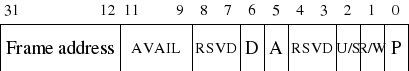
\includegraphics[width=10cm]{images/paging.png}
  \caption{Page Table entry format}
\end{figure}
Each process normally has a different set of page mappings, so that virtual memory spaces are independent of each other. In the x86 architecture (32-bit) pages are fixed at 4KB in size. Each page has a corresponding descriptor word, which tells the processor which frame it is mapped to. Note that because pages and frames must be aligned on 4KB boundaries (4KB being 0x1000 bytes), the least significant 12 bits of the 32-bit word are always zero. The architecture takes advantage of this by using them to store information about the page, such as whether it is present, whether it is kernel-mode or user-mode etc. The layout of this word is in the picture on the right.

The fields in that picture are pretty simple, so let's quickly go through them.
\begin{itemize}
  \item \textbf{P}: Set if the page is present in memory.
  \item \textbf{R/W}: If set, that page is writeable. If unset, the page is read-only. This does not apply when code is running in kernel-mode (unless a flag in CR0 is set).
  \item \textbf{U/S}: If set, this is a user-mode page. Else it is a supervisor (kernel)-mode page. User-mode code cannot write to or read from kernel-mode pages.
  \item \textbf{Reserved}: These are used by the CPU internally and cannot be trampled.
  \item \textbf{A}: Set if the page has been accessed (Gets set by the CPU).
  \item \textbf{D}: Set if the page has been written to (dirty).
  \item \textbf{AVAIL}: These 3 bits are unused and available for kernel-use.
  \item \textbf{Page frame address}: The high 20 bits of the frame address in physical memory.
\end{itemize}

\subsection{Page Faults}
When a process does something the memory-management unit doesn't like, a page fault interrupt is thrown. Situations that can cause this are (not complete):
\begin{itemize}
  \item Reading from or writing to an area of memory that is not mapped (page entry/table's 'present' flag is not set)
  \item The process is in user-mode and tries to write to a read-only page.
  \item The process is in user-mode and tries to access a kernel-only page.
  \item The page table entry is corrupted - the reserved bits have been overwritten.
\end{itemize}
The page fault interrupt is number 14, and looking at chapter 3 we can see that this throws an error code. This error code gives us quite a bit of information about what happened.
\begin{itemize}
  \item \textbf{Bit 0}: If set, the fault was not because the page wasn't present. If unset, the page wasn't present.
  \item \textbf{Bit 1}: If set, the operation that caused the fault was a write, else it was a read.
  \item \textbf{Bit 2}: If set, the processor was running in user-mode when it was interrupted. Else, it was running in kernel-mode.
  \item \textbf{Bit 3}: If set, the fault was caused by reserved bits being overwritten.
  \item \textbf{Bit 4}: If set, the fault occurred during an instruction fetch.
\end{itemize}
The processor also gives us another piece of information - the address that caused the fault. This is located in the CR2 register. Beware that if your page fault hander itself causes another page fault exception this register will be overwritten - so save it early!

\section{The VFS and the initrd}
\subsection{The virtual filesystem}
A VFS is intended to abstract away details of the filesystem and location that files are stored, and to give access to them in a uniform manner. They are usually implemented as a graph of nodes; Each node representing either a file, directory, symbolic link, device, socket or pipe. Each node should know what filesystem it belongs to and have enough information such that the relavent open/close/etc functions in its driver can be found and executed. A common way to accomplish this is to have the node store function pointers which can be called by the kernel. We'll need a few function pointers:
\begin{itemize}
  \item \textbf{Open} - Called when a node is opened as a file descriptor.
  \item \textbf{Close} - Called when the node is closed.
  \item \textbf{Read}
  \item \textbf{Write}
  \item \textbf{Readdir} - If the current node is a directory, we need a way of enumerating it's contents. Readdir should return the n'th child node of a directory or NULL otherwise. It returns a 'struct dirent', which is compatible with the UNIX readdir function.
  \item \textbf{Finddir} - We also need a way of finding a child node, given a name in string form. This will be used when following absolute pathnames.
\end{itemize}
So far then our node structure looks something like:
\begin{lstlisting}[style=CStyle]
  typedef struct fs_node
  {
     char name[128];     // The filename.
     u32int mask;        // The permissions mask.
     u32int uid;         // The owning user.
     u32int gid;         // The owning group.
     u32int flags;       // Includes the node type. See #defines above.
     u32int inode;       // This is device-specific - provides a way for a filesystem to identify files.
     u32int length;      // Size of the file, in bytes.
     u32int impl;        // An implementation-defined number.
     read_type_t read;
     write_type_t write;
     open_type_t open;
     close_type_t close;
     readdir_type_t readdir;
     finddir_type_t finddir;
     struct fs_node *ptr; // Used by mountpoints and symlinks.
  } fs_node_t;
\end{lstlisting}

\subsection{Mountpoints}
Mountpoints are the UNIX way of accessing different filesystems. A filesystem is mounted on a directory - any subsequent access to that directory will actually access the root directory of the new filesystem. So essentially the directory is told that it is a mountpoint and given a pointer to the root node of the new filesystem. We can actually reuse the ptr member of fs\_node\_t for this purpose (as it is currently only used for symlinks and they can never be mountpoints).
\begin{figure}[H]
  \centering
  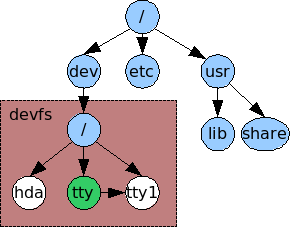
\includegraphics[width=12cm]{images/mount.png}
  \caption{devfs mounted on /dev}
\end{figure}

\subsection{The initial ramdisk}
An initial ramdisk is just a filesystem that is loaded into memory when the kernel boots. It is useful for storing drivers and configuration files that are needed before the kernel can access the root filesystem (indeed, it usually contains the driver to access that root filesystem!).\\
An initrd, as they are known, usually uses a propriatary filesystem format. The reason for this is that the most complex thing a filesystem has to handle, deletion of files and reclaimation of space, isn't necessary. The kernel should try to get the root filesystem up and running as quick as possible.
The initrd must load as a multiboot module.

\section{User mode}
Kernel mode makes available certain instructions that would usually be denied a user program - like being able to disable interrupts, or halt the processor.\\
Once you start running user programs, you'll want to make the jump from kernel mode to user mode, to restrict what instructions are available. You can also restrict read or write access to areas of memory. This is often used to 'hide' the kernel's code and data from user programs.
\begin{figure}[H]
  \centering
  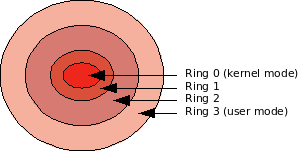
\includegraphics[width=8cm]{images/rings.png}
  \caption{devfs mounted on /dev}
\end{figure}
The x86 is strange in that there is no direct way to switch to user mode. The only way one can reach user mode is to return from an exception that began in user mode. The only method of getting there in the first place is to set up the stack as if an exception in user mode had occurred, then executing an exception return instruction (IRET).\\
The IRET instruction expects, when executed, the stack to have the following contents (starting from the stack pointer - the lowermost address upwards):
\begin{itemize}
  \item The instruction to continue execution at - the value of EIP.
  \item The code segment selector to change to.
  \item The value of the EFLAGS register to load.
  \item The stack pointer to load.
  \item The stack segment selector to change to.
\end{itemize}

The EIP, EFLAGS and ESP register values should be easy to work out, but the CS and SS values are slightly more difficult.\\
When we set up our GDT we set up 5 selectors - the NULL selector, a code segment selector for kernel mode, a data segment selector for kernel mode, a code segment selector for user mode, and a data segment selector for user mode.

They are all 8 bytes in size, so the selector indices are:
\begin{itemize}
  \item \textbf{0x00}: Null descriptor
  \item \textbf{0x08}: Kernel code segment
  \item \textbf{0x10}: Kernel data segment
  \item \textbf{0x18}: User code segment
  \item \textbf{0x20}: User data segment
\end{itemize}
We're currently using selectors 0x08 and 0x10 - for user mode we want to use selectors 0x18 and 0x20. However, it's not quite that straightforward. Because the selectors are all 8 bytes in size, the two least significant bits of the selector will always be zero. Intel use these two bits to represent the RPL - the Requested Privilege Level. These have currently been zero because we were operating in ring 0, but now that we want to move to ring three we must set them to '3'. If you wish to know more about the RPL and segmentation in general, you should read the intel manuals. There is far too much information for me to explain everything here.\\

The following snippet is to switch beetween the different mode:
\begin{lstlisting}[style=CStyle]
void switch_to_user_mode()
{
   // Set up a stack structure for switching to user mode.
   asm volatile("  \
     cli; \
     mov $0x23, %ax; \
     mov %ax, %ds; \
     mov %ax, %es; \
     mov %ax, %fs; \
     mov %ax, %gs; \
                   \
     mov %esp, %eax; \
     pushl $0x23; \
     pushl %eax; \
     pushf; \
     pushl $0x1B; \
     push $1f; \
     iret; \
   1: \
     ");
}
\end{lstlisting}

\bibliographystyle{abbrv}
\bibliography{simple}

\end{document}
